\subsection{Additional details for Experiment 2}
\label{appendix::exp2_holder}

This appendix gives the implementation details for the Hölder-smooth simulation in Experiment~2. The covariates are \(W=(W_1,\ldots,W_d)\), with independent coordinates drawn from \(U[-1,1]\). For a generated vector \(v=(v_1,\ldots,v_n)\), let \(\operatorname{Std}_n(v)\) denote empirical centering and scaling to mean zero and standard deviation one within that simulated dataset. Let \(a_j=j^{-3/4}/(\sum_{\ell=1}^d \ell^{-3/2})^{1/2}\). The additive score is
\[
  s_f(W)=\operatorname{Std}_n\left[
    \sum_{j=1}^d a_j\{\sin(\pi W_j)+0.5W_j^2+0.25\cos(2\pi W_j)\}
  \right].
\]
The rough score first includes univariate terms \(r_j(W)=\operatorname{sign}(W_j)|W_j|^{1/2}+0.25\sin(3\pi W_j)\). For \(d>1\), with \(\mathcal I_d=\{1,\ldots,\min(d,4)\}\), it also includes
\[
  \sum_{j<k,\ j,k\in\mathcal I_d}\sqrt{a_ja_k}
  \{\sin(\pi W_jW_k)+0.5\cos(\pi(W_j-W_k))\}
  +0.45\prod_{j\in\mathcal I_d}\tanh(1.5W_j)
  +\sum_{j\in\mathcal I_d}a_j\{0.35\,1(W_j>0.2)-0.25\,1(W_j<-0.45)\}.
\]
The pairwise and product terms are omitted when \(d=1\), retaining only the univariate rough and step terms. We denote the standardized rough score by \(s_s(W)\). The reported main-text regime sets
\[
  \eta_\pi(W)=\operatorname{Std}_n\{0.65s_f(W)+\sqrt{1-0.65^2}s_s(W)\},
  \qquad
  \eta_\mu(W)=s_f(W),
\]
so that both outcome logits are additive while the propensity score depends on the rough high-dimensional score. The treatment-effect score is \(s_\tau(W)=\operatorname{Std}_n\{0.75s_f(W)+0.25\sin(\pi W_1)\}\). The treatment and outcome mechanisms are
\[
  \pi_0(W)=\operatorname{clip}_{[0.03,0.97]}\{\operatorname{expit}(-0.2+1.15\eta_\pi(W))\},
\]
\[
  \mu_0(0,W)=\operatorname{expit}(-0.6+0.9s_f(W)),\qquad
  \mu_0(1,W)=\operatorname{expit}(-0.6+0.9s_f(W)+0.35+0.15s_\tau(W)),
\]
Given \(W\), treatment is Bernoulli with success probability \(\pi_0(W)\), and the binary outcome is Bernoulli with success probability \(\mu_0(A,W)\). The estimand is the ATE \(E\{\mu_0(1,W)-\mu_0(0,W)\}\).

For the XGB/RF runs in the main text, nuisance estimators are trained on an independent external sample with the same sample size as the analysis sample. The outcome regressions are estimated separately by treatment arm with depth-one \texttt{xgboost} using singleton interaction constraints, learning rate 0.1, up to 5000 boosting rounds, early stopping after 100 rounds, and a 20\% validation split. The propensity score is estimated with \texttt{ranger} probability forests using 500 trees, maximum depth 8, and \(mtry=\lfloor\sqrt d\rfloor\). Calibrated DML uses isotonic calibration, and the displayed calibrated interval is the level-set Wald interval.

The sample-size grid varies \(n\in\{2500,5000,10000,15000\}\) and \(d\in\{4,8,12,16\}\). The fixed-\(n\) dimension curve uses \(n=10{,}000\).

\begin{figure}[tbp]
     \centering
    \begin{subfigure}[b]{0.84\linewidth}
    \centering
    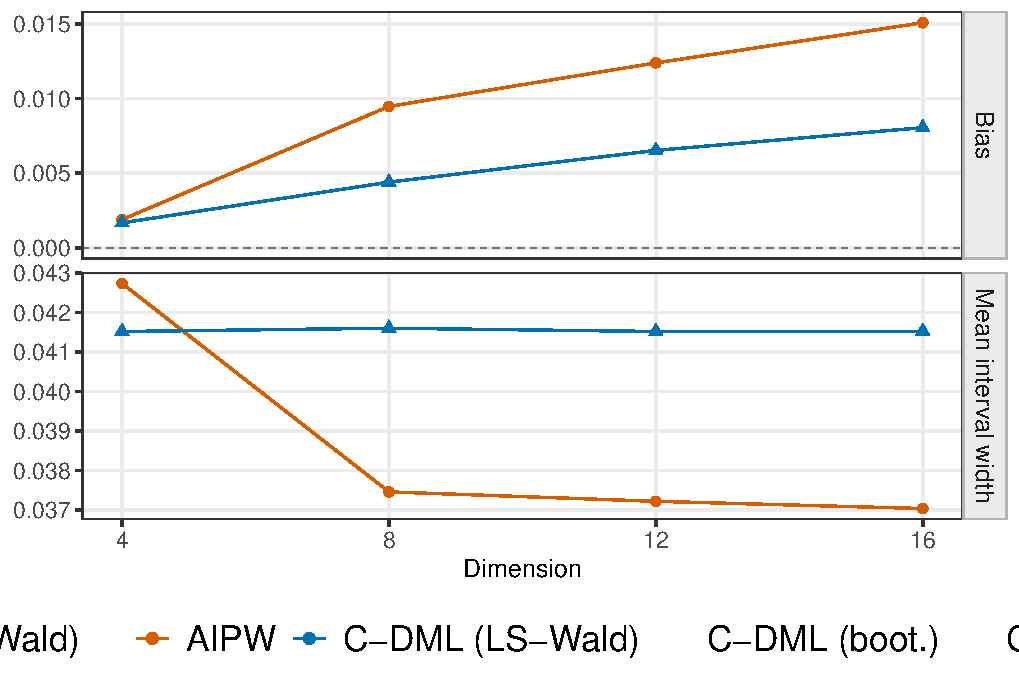
\includegraphics[width=\linewidth]{newplots/holder_exp2_dimcurve_n10000_xgbrf_bias_width.pdf}
    \subcaption{Dimension curve at \(n=10{,}000\).}
    \end{subfigure}
    \begin{subfigure}[b]{0.96\linewidth}
    \centering
    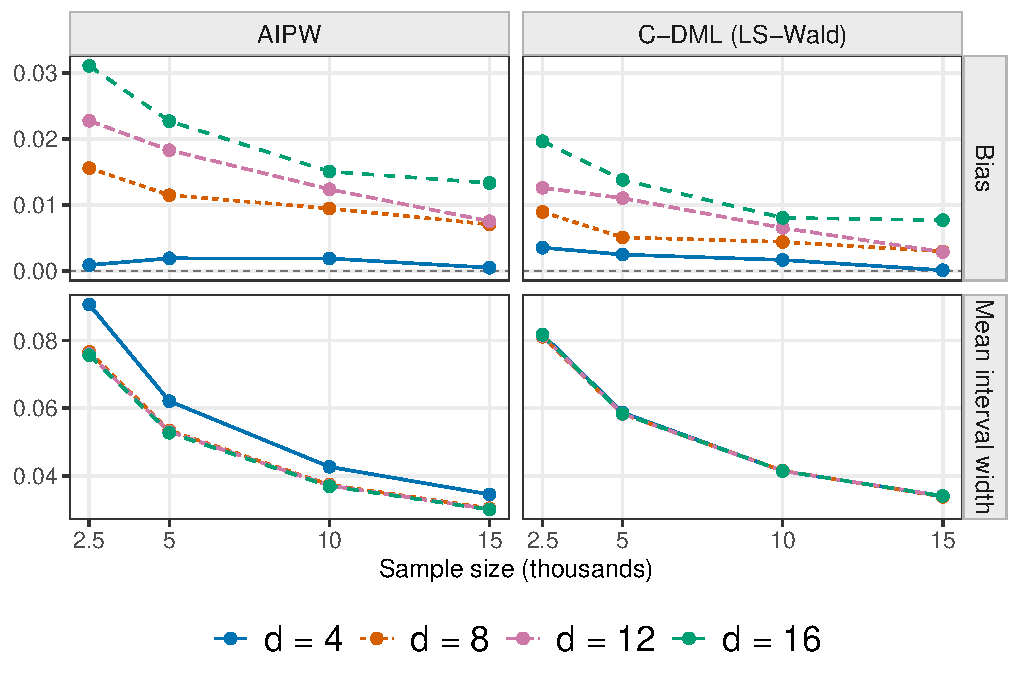
\includegraphics[width=\linewidth]{newplots/holder_exp2_samplegrid_external_xgbrf_bias_width_by_d.pdf}
    \subcaption{Sample-size grid with separate curves for each dimension.}
    \end{subfigure}
\caption{Empirical bias and interval width for the main XGB/RF Hölder-smooth simulation.}
       \label{fig::exp2_holder_bias_width}
\end{figure}

\begin{figure}[tbp]
     \centering
    \begin{subfigure}[b]{0.84\linewidth}
    \centering
    \includegraphics[width=\linewidth]{newplots/holder_exp2_appendix_dimcurve_n10000_glmnet_ridge_coverage_rmse.pdf}
    \subcaption{Dimension curve at \(n=10{,}000\).}
    \end{subfigure}
    \begin{subfigure}[b]{0.96\linewidth}
    \centering
    \includegraphics[width=\linewidth]{newplots/holder_exp2_appendix_samplegrid_glmnet_ridge_nsim100_coverage_rmse_by_d.pdf}
    \subcaption{Sample-size grid with separate curves for each dimension.}
    \end{subfigure}
\caption{Appendix comparison using additive lasso outcome regression and high-dimensional ridge propensity regression in the same Hölder-smooth design.}
       \label{fig::exp2_holder_glmnet}
\end{figure}
